\documentclass{sigchi}
% Remove or comment out these two lines for final version
\toappearbox{\Large Submitted to IUI'13. \\Do not cite, do not circulate.}

% Arabic page numbers for submission. 
% Remove this line to eliminate page numbers for the camera ready copy
%\pagenumbering{arabic}

% Load basic packages
\usepackage{balance}  % to better equalize the last page
\usepackage{graphics} % for EPS, load graphicx instead
\usepackage{times}    % comment if you want LaTeX's default font
\usepackage{url}      % llt: nicely formatted URLs
\usepackage{subfigure}

% llt: Define a global style for URLs, rather that the default one
\makeatletter
\def\url@leostyle{%
  \@ifundefined{selectfont}{\def\UrlFont{\sf}}{\def\UrlFont{\small\bf\ttfamily}}}
\makeatother
\urlstyle{leo}

% To make various LaTeX processors do the right thing with page size.
\def\pprw{8.5in}
\def\pprh{11in}
\special{papersize=\pprw,\pprh}
\setlength{\paperwidth}{\pprw}
\setlength{\paperheight}{\pprh}
\setlength{\pdfpagewidth}{\pprw}
\setlength{\pdfpageheight}{\pprh}
\hyphenpenalty=750 % for preventing too make words breaking into separate lines

% Make sure hyperref comes last of your loaded packages, 
% to give it a fighting chance of not being over-written, 
% since its job is to redefine many LaTeX commands.
\usepackage[pdftex]{hyperref}
\hypersetup{
pdftitle={SIGCHI Conference Proceedings Format},
pdfauthor={LaTeX},
pdfkeywords={SIGCHI, proceedings, archival format},
bookmarksnumbered,
pdfstartview={FitH},
colorlinks,
citecolor=black,
filecolor=black,
linkcolor=black,
urlcolor=black,
breaklinks=true,
}

% create a shortcut to typeset table headings
\newcommand\tabhead[1]{\small\textbf{#1}}

% End of preamble. Here it comes the document.
\begin{document}

% ##############################
% # TITLE
% ##############################

\title{HaptiGo: An Intelligent and Lightweight Tactile Vest for Improving Active Pedestrian Navigation Experiences}

% ##############################
% # AUTHORS LIST
% ##############################

\numberofauthors{2}
\author{
  \alignauthor Anonymous\\
    \affaddr{...}\\
    \affaddr{...}\\
    \email{...}\\
    \affaddr{...}
}

% Teaser figure can go here
%\teaser{
%  \centering
%  \includegraphics{Figure1}
%  \caption{Teaser Image}
%  \label{fig:teaser}
%}

\maketitle

% ##############################
% # ABSTRACT
% ##############################

\begin{abstract}
Pedestrians can seamlessly navigate within familiar environments to their intended destinations by advantageously tapping into their prior knowledge of their surroundings. Yet, when pedestrians are in unexplored environments or are engaged in other tasks, these benefits are lost as they must take on greater awareness of their surroundings, or take on higher cognitive loads, respectively. We propose HaptiGo, a lightweight haptic vest which provides navigation intelligence and is capable of guiding pedestrians to their intended destinations and away from potential obstacles. The HaptiGo system consists of well-placed vibro-tactile sensors that utilize natural and small form factor interaction cues which emulate the invisible sensation of being passively guided in the right direction. We individually evaluated our vest on a group of pedestrians navigating through several different waypoints while engaged in cognitively demanding tasks, and our results demonstrated that users navigated to their destinations effectively and enjoyed our haptic interface solution.
\end{abstract}

% ##############################
% # AUTHOR KEYWORDS
% ##############################

\keywords{
    Mobile user interface, haptics, tactile display, pedestrian navigation, intelligent fabrics.
}

% ##############################
% # ACM CLASSIFICATION KEYWORDS
% ##############################

\category{H.5.2.}{User Interfaces}{Haptic I/O}

% ##############################
% # INTRODUCTION
% ##############################

\section{INTRODUCTION}
As people navigate from one location to another by foot, they can take advantage of prior knowledge of their surroundings to guide themselves towards their intended destinations.  Greater familiarity in their environments from this prior knowledge also enables people to engage in multi-tasking while making the most of their available time, alleviating any boredom, and so on.  These parallel tasks in conjunction with navigation are also quite diverse in scope and can range from social activities, such as engaging in serious discussion with colleagues, casually texting with a friend, or talking to family on the phone; to more personal activities, such as listening to music with headphones, browsing information on a smartphone, or playing video games on a portable gaming device.

These habits subsequently introduce two distinct challenges as people grow accustomed to multi-tasking while navigating familiar environments: the challenge of inconvenience where people must become more aware of their surroundings and navigation tools in unfamiliar environments due to lack of prior knowledge, and the serious challenge of exposing people to greater danger while navigating in more active environments \cite{2010_Madden_PewResearch}.  While the former challenge is readily apparent, the latter challenge occurs especially to individuals who suffer from situation-induced impairments \cite{2007_Jupp_UAHCI}, which is when they lose awareness about the situation around, such as through secondary tasks and self-imposed distractions when multi-tasking during pedestrian navigation.  Examples include frequent cases of people bumping into others while their attention is focused on their mobile devices \cite{2010_Madden_PewResearch}, and the loss of situational awareness (i.e., \textit{iPod Zombie trance}) while listening to loud music that have also led to rising rates of pedestrian fatalities \cite{2012_Pielot_CHI}.

Conventional navigation systems found on multitudes of mobile devices -- especially those which typically rely on either visual or auditory modalities -- prove lacking when it comes to addressing the specifics from these particular challenges.  In response, various studies have shown the effectiveness of navigation solutions which instead utilize alternate tactile modalities, especially when users are cognitively occupied in performing other tasks \cite{2010_Elliott_IEEEHaptics}.  Moreover, touch provides great appeal in communicating navigation information without simultaneously introducing mental distraction, since tactile sensory channels are hardly affected when utilized to observe people’s surroundings \cite{2012_Pielot_CHI}.  According to related theoretical frameworks \cite{2010_Elliott_IEEEHaptics, 2002_Wickens_ErgoScience}, the tactile modality has great appeal as it can “serve to guide, reduce workload, and support situation and navigation performance”.

There is great potential in developing an effective tactile navigation system which supports the types of behaviors contained in these challenges.  We therefore propose HaptiGo, a lightweight haptic vest which provides navigation intelligence of tactilely guiding pedestrians to their intended destinations and away from potential obstacles through well-placed vibro-tactile sensors, while providing natural and small form factor interaction cues which emulate the invisible sensation of being passively guided in the right direction. We individually evaluated our vest on a group of pedestrians navigating through several different waypoints while engaged in cognitively demanding tasks, and our results demonstrated that users navigated to their destinations effectively and enjoyed our haptic interface solution.

\subsection{Design Constraints}
In order to design an intelligent user interface for pedestrian navigation that addressed our proposed challenges, we first had to explore design constraints that both intelligently and intuitively navigated users.  The interaction analogy that inspired our design of HaptiGo was that of a friendly guide whom physically nudged the user towards the right direction and away from potential hazards.

\textit{Tactile Feedback}\\
One analogy that we explored and expressed interest in involved interaction cues which emulated the physical action of appropriately nudging users during navigation.  That is, an interaction that emulated a guide reaching out to the user and physically directing them in a friendly manner.  In this case, we desired a tactile interface which provided feedback on the user's upper torso area, since it was an ideal region for providing emulated interaction cues in nudging a person towards and away from points of interest.

\textit{Navigation Guidance}\\
Once we established on a desired model of the tactile feedback, we needed to decide on interaction cues which serve to guide the users effectively and intuitively.  The analogy that we sought was one where a guide would gently nudge users to the desired area, such as tapping the user from behind towards the intended direction.

\textit{Obstacle Avoidance}\\
The complementary interaction of guiding users towards their target would be in guiding users away from potential hazards, so we also needed to decide on interaction cues to express that type of behavior.  The analogy that interested us was a guide whom would reach out in front of the user and block the user from progressing any further due to an incoming hazard.

\subsection{Example Scenarios}
Our system is designed for scenarios where the users are engaged in multitasking while navigating. Th ser isn tsuch scenarios use passive awareness ofh the environment to navigate. The following scenarios illustrate the situations where a user could take advantage of our system. George is a paratrooper in airborne troops. He is on an operation that involves him to parachute into enemy territory with other Soldiers. Once he has landed, he has to reorient himself and find his way to the rendezvous point. Since he is in an hostile terrain, he should maintain awareness about the space around him, maintain his stealth and navigate through the unfamiliar terrain. George could use HaptiGo to offload the cognitive task of navigation while maintaining an awareness of the space around him.

Stacy is a player of the game called geocaching. The game involves Stacy finding hidden treasure at a given location. The latitude and longitude of the treasure is specified in the game. Stacy would have to navigate to this location and search for treasure in an unfamiliar terrain. Stacy could use our HaptiGo system to help her find obstacle on her path and navigate through the terrain while she is engaged in finding the treasure given at the location.

Maggie is an undergraduate student in a university. She has just finished her class in building A and has a class in building B. She receives a text from her friend. While she is typing a reply to her friend, she has to walk to building B through a route that is busy with students. Maggie could use our system to help her multi-task while walking from building A to B. HaptiGo will help her navigate through the crowded route augmenting her awareness of the environment which is decreased while texting.
% ##############################
% # RELATED WORK
% ##############################

\section{RELATED WORK}
Research work as far back as over a decade ago \cite{2000_Ross_ASSETS} has focused on the development of pedestrian navigation systems that either additionally included or alternatively incorporated tactile modalities. While not primarily targeting people with situation-induced impairments, such systems have been developed to accommodate various other pedestrian types such as tourists in unfamiliar environments (e.g., \cite{2012_Pielot_CHI, 2012_Szymczak_MobileHCI}), soldiers in sensitive environments (e.g., \cite{2012_Cummings_CHINZ, 2010_Elliott_IEEEHaptics}), and vision-impaired individuals in bustling environments (e.g., \cite{2006_Johnson_EMBS, 2010_Pielot_Pervasive}). Furthermore, these systems propose diverse solutions which take full advantage of tactile modalities in pedestrian navigation, ranging from mobile user interfaces which exploit mobile communication devices' vibration alerts to wearable tactile displays such as vibrotactile belts and vests.

\subsection{Mobile User Interfaces}
The global ubiquity of mobile devices such as the recent generation of smartphones have motivated researchers to build multitudes of mobile navigation apps with tactile feedback support by taking advantage of those mobile devices' built-in vibrating alert feature.  These various solutions provide their own approaches that build upon the existing capabilities of mobile phone technologies and can be categorized into two different types: \textit{magic wand} and \textit{sixth sense}~\cite{2011_Frohlich_CommunACM}.

\textit{Magic Wand}\\
Mobile user interfaces which incorporate \textit{magic wand} functionality take their cues from the metaphor of pointing the device at a distant object to learn more about its presence and access its corresponding information~\cite{2011_Frohlich_CommunACM}, and have been made specifically more feasible with recent mobile devices such as smartphones due to increased built-in digital compass capabilities ~\cite{2012_Pielot_CHI}. In the context of pedestrian navigation, mobile user interfaces which incorporate \textit{magic wand} functionality have recently been utilized to actively scan the user's surroundings, such as physically waving the mobile device with their arms stretched out forward or turning their bodies around with the mobile device in their possession~\cite{2010_Magnusson_HAID, 2010_Magnusson_MobileHCI}, and for different purposes, such as better guidance for the visually-impaired individuals \cite{2010_Magnusson_NordiCHI}, more flexible routes for exploring tourists \cite{2010_Robinson_MobileHCI}, and improved streamlined meetups for social groups \cite{2010_Williamson_CHI}.

These \textit{magic wand} interfaces have proven successful in terms of intuitiveness from user feedback, and evaluations from these cited examples have demonstrated that users are able to reach target destinations effectively (e.g., \cite{2010_Magnusson_HAID, 2010_Robinson_MobileHCI, 2010_Williamson_CHI}).  While these systems benefit interface pedestrians through more intuitive navigation through a \textit{magic wand} metaphor, this intuitiveness comes at the cost of requiring users to be actively engaged with these interfaces \cite{2010_Robinson_MobileHCI}.  Consequently, not only would this type of interaction be cumbersome and exhausting to users over prolonged use as they adjust their limbs or bodies while locating their target destinations, but users with situation-induced impairments would not be able to benefit from such interfaces as they would require active engagement with these interfaces.

\textit{Sixth Sense}\\
Alternative techniques to the \textit{magic wand} metaphor have instead adopted a \textit{sixth sense} metaphor, which describes the interaction technique of using multimodal feedback to alert the user about changes within the environment~\cite{2011_Frohlich_CommunACM}.  In the context of pedestrian navigation, \textit{sixth sense}-based interfaces enable users to derive the location of their target destinations in relation to their current location and orientation~\cite{2012_Pielot_CHI}.

Techniques that rely on the \textit{sixth sense} metaphor have provided their own implementations either through turn-by-turn-based vibration patterns (e.g., \cite{2008_Lin_OZCHI, 2012_Raisamo_EuroHaptics}) or compass-based directional vibration cues (e.g., \cite{2012_Cummings_CHINZ, 2011_Pielot_ICMI, 2011_Pielot_INTERACT, 2011_Rumelin_UIST, 2012_Szymczak_MobileHCI}).  In comparison to \textit{magic wand} interfaces, \textit{sixth sense} interfaces benefit users through more passive interaction; in other words, users are not required to search for spatial entities by explicitly performing pointing gestures.  Consequently, the lack of such active gesturing to physical directions in \textit{sixth sense} interfaces means that these interfaces are less intuitive and possess a steeper learning curve.  As a result, users must first understand the directional meaning of the mobile devices' vibration feedback (e.g., meaning of vibration patterns, context of vibration cues) before they may be able to successfully navigate to their target destinations.

\textit{Magic Wand + Sixth Sense}\\
Insights extracted from the contributions of these existing tactile-based mobile user interfaces have enabled researchers to explore possible synergies in a hybrid technique of both \textit{magic wand} and \textit{sixth sense}, such as applying vibration patterns from \textit{magic wand} techniques that also expressed the direction of target destinations relative to the mobile device found in \textit{sixth sense} techniques (e.g., \cite{2010_Magnusson_HAID, 2010_Pielot_MobileHCI, 2011_Pielot_ICMI}).  Efforts from these explorations demonstrated that improvements were achievable for interfaces combining the strengths of both \textit{magic wand} and \textit{sixth sense} techniques; these subsequent interfaces accomplished the intuitive strengths of \textit{magic wand} techniques with the passive capabilities of \textit{sixth sense} interfaces without requiring that pointing gestures be executed.

While more recent navigation interfaces enjoy the benefits in \textit{magic wand} and \textit{sixth sense} techniques, one limitation that the hybrid technique possessed stemmed from evaluations which demonstrated lingering intuitiveness issues such that users required further training in order to utilize tactile feedback for pedestrian navigation~\cite{2012_Pielot_CHI}.  Moreover, theoretical frameworks revealed that the placement of tactile information was critical to be intuitively comprehended by users~\cite{2010_Elliott_IEEEHaptics, 2007_VanErp_Dissertation}; in the case of the hybrid technique, this tactile information is singularly expressed from the vibrating alarm of the mobile device which less effectively and intuitively conveys navigation information when carried by hand or in clothing compared to techniques which incorporate additional and more optimally placed tactile sensors (e.g., tactile displays).  An additional limitation of the hybrid technique stems from the hardware (i.e., the mobile device's vibrating alarm) used for expressing tactile information when additionally including obstacle detection; further intuitiveness issues may develop from the ambiguity of determining whether cues from the vibration alarm indicate either navigation guidance or obstacle detection.

\subsection{Wearable Tactile Interfaces}
While tactile mobile user interfaces for pedestrian navigation have experienced greater developments following the growing ubiquity of smartphones and more advanced feature phones \cite{2012_Pielot_CHI}, earlier tactile navigation systems consisted of wearable tactile interfaces (e.g., \cite{2000_Ross_ASSETS, 2004_Tsukada_Ubicomp}) which continued evolving in terms of smaller form factor and improved intuitiveness (e.g., \cite{2011_Elliott_HI, 2010_Pielot_Pervasive}).  Wearable tactile interfaces are also not constrained to a single vibrotactile sensor (i.e., vibrating alarm) on mobile phones like in mobile user interfaces, so these interfaces also enable richer feedback (e.g., more sensors, more optimal placement of interface) and greater flexibility (e.g., less constraints on placement of interface).  Recent technological advances and near-future ubiquitious possibilities of intelligent fabrics (e.g., \cite{2008_Buechley_CHI}) have further made wearable tactile interfaces viable options for providing tactile navigation assistance. Various earlier wearable tactile interfaces proposed placing devices on different regions of the body, ranging from the upper body (e.g., head, shoulders, torso) to the lower body (waist, feet), and researchers have reported that the most successful interfaces were specifically placed either on the waist (i.e., tactile belts) or on the torso (i.e., tactile vests) ~\cite{2010_Srikulwong_HAID}.

\textit{Tactile Belts}\\
Various proposed tactile belts systems for pedestrian navigation share similar characteristics in embedding vibrotactile sensors around the waist which generate absolute point pulses analogous to receiving visual from a compass \cite{2010_Srikulwong_HAID}.  Earlier tactile belt prototypes (e.g., \cite{2004_VanVeen_EuroHaptics, 2005_VanErp_TAP, 2006_Johnson_EMBS, 2005_Nagel_JNeuralEng, 2004_Tsukada_Ubicomp} provided tactile feedback on larger, protruding belts that guided users with navigational feedback from a backpack-carried laptop or nearby server, while more recent tactile belt systems (e.g., \cite{2010_Pielot_Pervasive, 2009_Pielot_MobileHCI}) achieved small form factors similar to clothing belts and with navigational guidance from GPS-enabled smartphones.

Some of the advantages demonstrated by tactile belt designs included users intuitively understanding the direction cues from the tactile feedback \cite{2005_VanErp_TAP} and performing better compared to wearing early-generation pattern-based tactile vests in controlled studies~\cite{2010_Srikulwong_HAID}.  An observation we made with tactile belt designs though involved additionally incorporating obstacle detection functionality; since sensors on existing tactile belt systems are equally-spaced around the user's waist, this introduced the possibility of usability issues of interpreting what tactile feedback would indicate navigational cues and what would indicate obstacle avoidance.

\textit{Tactile Vests}\\
Wearable tactile interfaces for pedestrian that are alternative to tactile belts are tactile vests, which consist of torso vests and embedded with a set of vibrotactile sensors; early-generation vests were bulkier and supported sensors which generated straight-line patterns (e.g., directional gestures) \cite{2004_Jones_HAPTICS, 2000_Ross_ASSETS} which functioned as pulsating sequences, while more recent vests were better streamlined and supported relative point vibrations on the backside of the user (e.g., left, forward, right) \cite{2012_Cummings_CHINZ, 2010_Elliott_IEEEHaptics, 2011_Elliott_HI} during navigation.

Recent tactile vest approaches have demonstrated advantages including their effectiveness in displaying direction cues based on both controlled and preliminary field studies \cite{2010_Elliott_IEEEHaptics} and in navigating users without distracting them \cite{2010_Pielot_Pervasive}.  Moreover, various theoretical frameworks (e.g., Wickens' Multiple Resource Theory \cite{2002_Wickens_ErgoScience}, van Erp's Prenav model \cite{2007_VanErp_Dissertation}) provide supporting evidence on the effectiveness of tactile vests in improving various aspects of navigation.  The Prenav model particularly theorizes that simply providing tactile information in navigation is not enough, and observations have shown that direction information can be intuitively comprehended with torso-placed sensors such as on tactile vests  \cite{2010_Elliott_IEEEHaptics}.  While the cited works on tactile vests focus specifically on pedestrian navigation tasks, the tactile vest approach specifically appealed to us due to their supported intuitive benefits and also provided design constraints which supported both navigation guidance and obstacle avoidance functionality through more natural interaction cues.

% ##############################
% # IMPLEMENTATION
% ##############################

\section{IMPLEMENTATION}
The Haptigo System consists of a LilyPad Arduino \cite{Arduino}, a Nexus One Android smartphone \cite{Android}, the BlueSmirf Bluetooth module \cite{BlueSmirf}, an Ultrasonic Ping Sensor \cite{PingSensor}, and five LilyPad Vibe Boards ( vibrational tactors) \cite{VibeBoard}. Figure \ref{fig:haptigoschematic} shows a schematic diagram of the components used in the system. The haptigo system has two functionality - navigation and obstacle detection. 

\begin{figure}[ht]
\centering
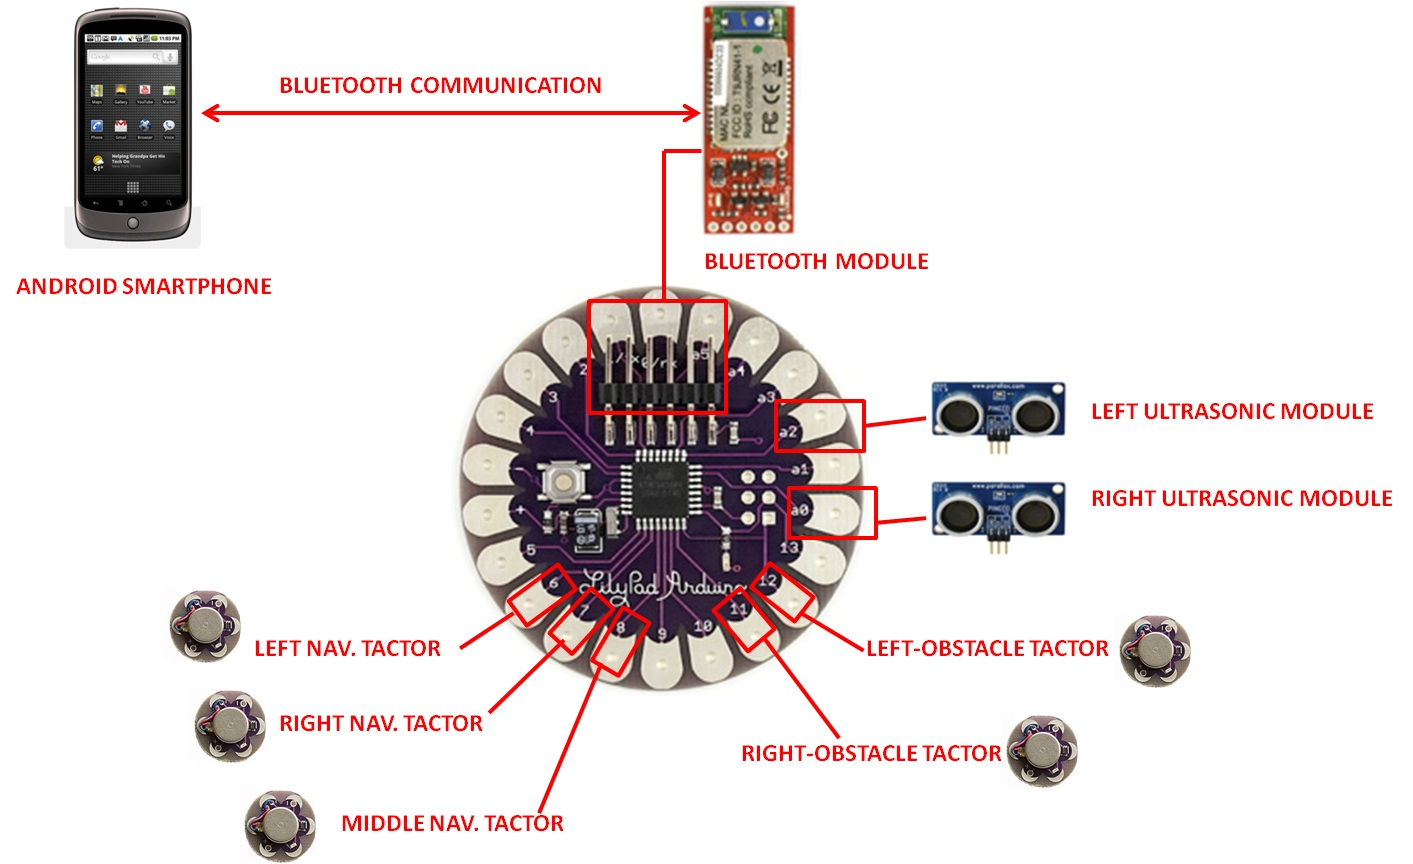
\includegraphics[width=0.9\columnwidth]{Images/Complete_System_Diagram.jpg}
\caption{Schematic diagram of the components used in Haptigo.}
\label{fig:haptigoschematic}
\end{figure}

\subsection{Navigational Feedback}
To implement the navigation functionality of the Haptigo system, we used an Android smartphone \cite{Android} as a source of location updates (GPS), as a measure of the alignment of the user (magnetometer) and also as, a processing unit (for calculating the directional cues). The directional cues calculated by Android \cite{Android} were communicated to the Lilypad Arduino \cite{Arduino} by using the Bluesmirf \cite{BlueSmirf}, bluetooth chip. The Lilypad Arduino \cite{Arduino} in turn activates one of the three vibrational tactors that gives directional cues.

We use three vibrational tactors for conveying navigational information. One vibrational tactor for suggesting left turn, one for right turn and one for going straight.  Three vibrational tactors are arranged in a “Y” pattern on the left back shoulder, right back shoulder and the center back of the wearer. All the three vibrational tactors are situated on the back side of user’s torso. Figure \ref{subfigure:haptigo:back:mold} illustrates the position of tactors on back side of torso. This arrangement was found to be intuitive as users instinctively turned left when the left tactor was activated, and turned right when the right tactor was activated.

\begin{figure}
\centering
\subfigure[Position of vibrational tactors used for navigation in Haptigo.]{
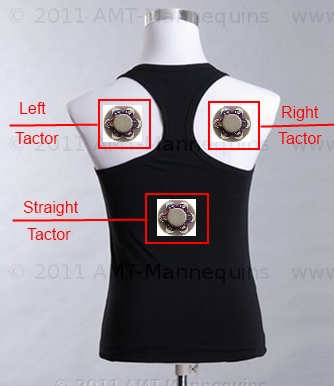
\includegraphics[width=0.45\columnwidth]{Images/HaptigoSystem_Back.jpg}
\label{subfigure:haptigo:back:mold}
}
\subfigure[Rear view of user wearing Haptigo vest.]{
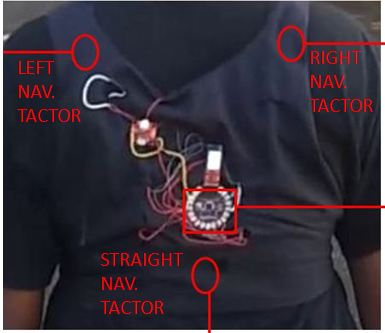
\includegraphics[width=0.45\columnwidth]{Images/Haptigo_BackView.JPG}
\label{subfigure:haptigo:back:real}
}
\caption{Rear view of haptigo vest.}
\label{figure:haptigo:back}
\end{figure}

A directional haptic cue is encoded as three distinct, consecutive vibration pulsed 0.5 seconds apart. The direction to turn is conveyed to the user by the location of the vibrating tactor i.e. a vibrating tactor on the left shoulder indicates the wearer should begin a left turn, a vibrating tactor on the right shoulder indicates a right turn, and lastly a vibrating tactor in the center of the back indicates the wearer should keep on straight.

We chose pulses based on our feedback from initial pilot study. A continuous vibrational feedback was interpreted as a push and a pulsed vibrational signal was interpreted as tap on the shoulder. The continuous and pulsed signals stimulate opposite responses from the user. A continuous vibrational signal on the right shoulder would make the user turn left because s/he would interpret it as someone pushing him/her in the counterclockwise direction. A pulsed signal on the right shoulder would make the user turn right because s/he interprets it as someone tapping him/her on right shoulder. This evokes the user to turn right.

\subsection{Obstacle Detection}
The second functionality of our system was to alert the wearer to approaching obstacles within his/her immediate vicinity. Two ultrasonic ping sensors \cite{PingSensor} are used to find obstacles in the user’s vicinity. The ping sensors are placed just below the user’s neck. One sensor is placed to the left just above the user’s chest and another sensor is placed to the right just above the user’s right chest. The left sensor detects obstacles approaching the users from his/her left and the right sensor detects the obstacles approaching the users from his/her right. The Lilypad Arduino \cite{Arduino} reads the input from two ultrasonic ping sensors, detects the existence of an obstacle and calculates the movement of the obstacle relative to the user. 

\begin{figure}
\centering
\subfigure[Position of vibrational tactors used for obtacle detection in Haptigo.]{
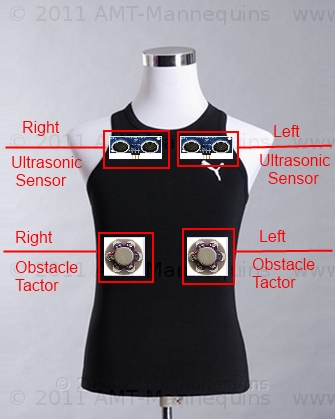
\includegraphics[width=0.45\columnwidth]{Images/HaptigoSystem_Front.jpg}
\label{subfigure:haptigo:front:mold}
}
\subfigure[Front view of user wearing Haptigo vest.]{
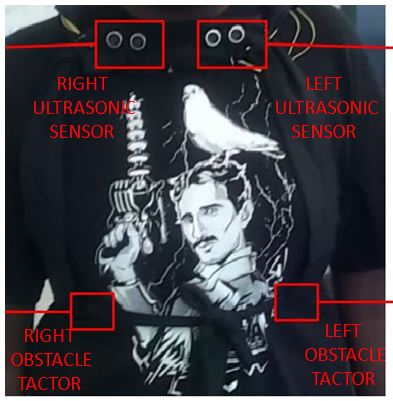
\includegraphics[width=0.45\columnwidth]{Images/Haptigo_FrontView.JPG}
\label{subfigure:haptigo:front:real}
}
\caption{Front view of haptigo vest.}
\label{figure:haptigo:front}
\end{figure}

The LilyPad Arduino activates either of the two vibrational tactors to notify the users, The two vibrational tactors are placed just below right and left user’s chest area. An approaching obstacle on the right is alerted using right vibrational tactor and an approaching obstacle on the left is alerted using left vibrational tactor. A haptic cue for an obstacle is encoded as one vibrational pulse of 1 second. We have designed the system to alert users when the obstacles are approaching. The system does not alert the user when an obstacle is detected. It alerts the user when an obstacle moves closer to the user. Figure \ref{subfigure:haptigo:front:mold} illustrates the position of tactors on front side of torso.


% ##############################
% # Evaluation
% ##############################

\section{EVALUATION}
We performed two studies to evaluate our system - a pilot study with four users and a user study with ten users. There was one female participant and three male participants in the pilot study. In the user study, we had two female participants and eight male participants.

In the pilot study, the users wore the haptigo vest and then were directed along a pre-determined route. The route consisted of one right turn and one left turn. Figure \ref{figure:pilot:route} shows the route used in the pilot study. The starting and ending points of the pilot study are illustrated with an 'X' symbol. In addition to testing the system functionality, we collected feedback from the user regarding the intuitiveness of the haptic cues used in the system.

\begin{figure}[ht]
\centering
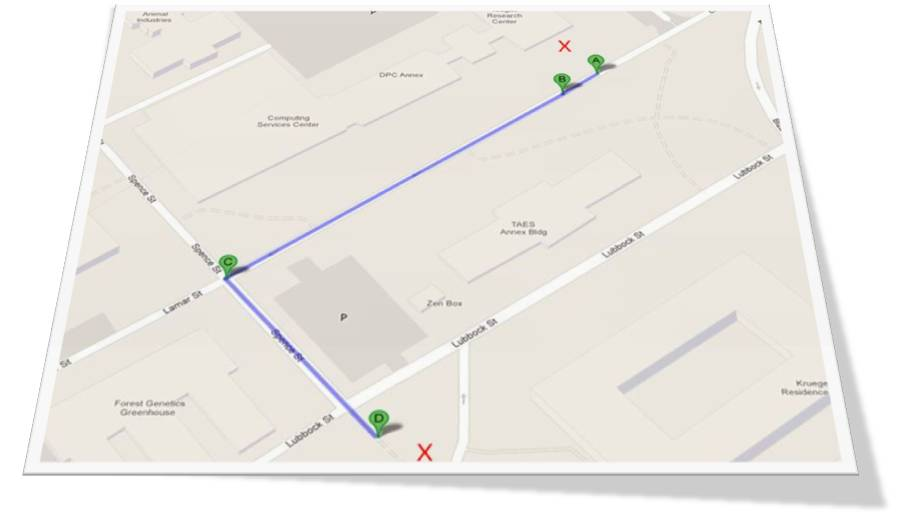
\includegraphics[width=0.8\columnwidth]{Images/PilotStudyRoute.JPG}
\caption{Route taken by participants in pilot study.}
\label{figure:pilot:route}
\end{figure}

In our user study, we compared our system against PocketNavigator\cite{2010_Pielot_MobileHCI}. PocketNavigator\cite{2010_Pielot_MobileHCI}, an Android application, uses vibrational tactor in the smartphone to provide haptic cues for direction. Figure \ref{figure:pocketnavigator} illustrates the haptic cues used by PocketNavigator\cite{2010_Pielot_MobileHCI} for each direction. The haptic cue for straight is two consecutive short pulse, the haptic cue for left is one long pulse followed by a short pulse, the haptic cue for right is a short pulse followed by a long pulse and the haptic cue for turning back is three consecutive short pulses. The length of vibration, the order of vibrational pulses and the number of pulses in a haptic cue is used to differentiate the direction.

\begin{figure}[ht]
\centering
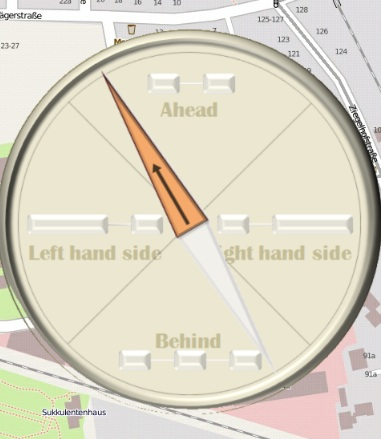
\includegraphics[width=0.5\columnwidth]{Images/PocketNavigator.jpg}
\caption{Directional cues presented by PocketNavigator, Android app.}
\label{figure:pocketnavigator}
\end{figure}

We used the following scenario to compare Haptigo with PocketNavigator\cite{2010_Pielot_MobileHCI}. A user wants to navigate from building A to building B in his university. While walking to the destination, she needs to type in a text using her smartphone. She opens up the Haptigo/ PocketNavigator\cite{2010_Pielot_MobileHCI} app in her smartphone. Types in the destination. She uses Haptigo/ PocketNavigator\cite{2010_Pielot_MobileHCI} to help her navigate to the destination while texting on her way to building B.

The navigation route was predetermined in our User study. Figure \ref{figure:userstudy:route} shows the route taken by the user for user study. As before with the pilot study image, the starting and ending points are illustrated with an 'X' symbol. We designated a starting and ending point for all users. The predetermined route was setup to ensure that a large amount of obstacles (pedestrians, and construction equipment) would be included in the path. In order to avoid familiarity of the user with a particular route, waypoints were setup as mandatory checkpoints before the destination could be reached. This mandatory checkpoint was implemented to be transparent to the user of the Haptigo System .In our scenario, texting is used as the secondary task. Every user in this study will have to navigate from point A to point B while texting. The experimenter will provide the text to be typed.

\begin{figure}[ht]
\centering
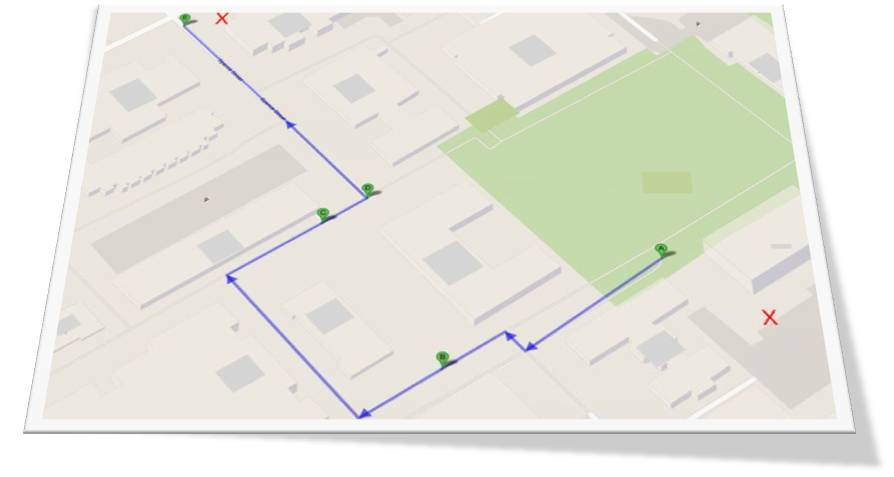
\includegraphics[width=0.8\columnwidth]{Images/UserStudyRoute.JPG}
\caption{Route taken by participants in user study.}
\label{figure:userstudy:route}
\end{figure}

Each user in the user study was given training with both the PocketNavigator\cite{2010_Pielot_MobileHCI} and Haptigo systems. In the case of PocketNavigator\cite{2010_Pielot_MobileHCI}, the user was trained to decipher the vibration signals output by the phone. In the case of the Haptigo system, users went through a calibration step. In the calibration step, each of the five vibrational tactors were activated in order to teach the user how to decipher these signals. After the calibration step, users demonstrated an understanding that the vibrational tactors located in the back of the Haptic Vest signaled directional cues while the  vibrational tactors located in the front of the Haptic Vest signaled obstacle cues.

The user performed the navigation task twice. Once with PocketNavigator\cite{2010_Pielot_MobileHCI} and the other time with the Haptigo system. The route taken between points A and B for PocketNavigator\cite{2010_Pielot_MobileHCI} and Haptigo were different. However, the number of waypoints situated in the route along with the route length were kept approximately equal for the routse used in the PocketNavigator\cite{2010_Pielot_MobileHCI} and Haptigo System.

The Independent Variable in the user study was the navigation system that was used. The Dependent Variables were the typing rate of users, and the time taken by the user to move from point A to B. At the end of the user study,  users filled a questionnaire asking users to rate their experience with the system on a five-point likert scale. The users rated each of the systems based on the following metrics: ease of use in navigation, haptic cues for navigational directions, and haptic cues for approaching obstacles (if applicable). Any subjective feedback from the user about the system was recorded.

% ##############################
% # RESULTS
% ##############################

\section{RESULTS}
We collected feedback from four users in our pilot study. In our initial system, haptic cues for direction were encoded as a single continuous signal. For example: If the intended navigation direction was to the right, the vibrational tactor at the right-back shoulder would turn on for one second. Two of the users felt such a feedback was equivalent to a push from the back causing the users to make a left turn instead of right. This feedback from the users prompted a change in the duration of the haptic cues from one continuous pulse to three consecutive pulse spaced 0.5 seconds apart. The consecutive haptic cues were considered by users to be similar to taps on the shoulder rather than push. So a haptic cue on the right shoulder had the user turn right.

A third user stated that the haptic cues for obstacles were unintuitive. In our initial system, users were alerted when the system detected an obstacle. Our third user remarked that, It is more intuitive to know if an obstacle is approaching me than an obstacle which is either stationary or moving away from me. Based on this feedback, we changed our system where it detects the movement of obstacle relative to the user. The system then notifies the user when the obstacle moves closer relative to the user.

We collected navigation time and typing rate data from the user study. We also collected ease of use and feedback on directional cues in Haptigo and PocketNavigator\cite{2010_Pielot_MobileHCI}. The mean and standard deviation for navigation time and typing rate are provided in Table \ref{table:navigationtime:typingrate}. Figure \ref{figure:haptigo:navigationtime} shows the distribution of navigation time across ten participants and Figure \ref{figure:haptigo:typingrate} shows the distribution of typing rate across ten users. One user did not want to do the typing task when she performed navigation using PocketNavigator\cite{2010_Pielot_MobileHCI}. She stated it was inconvenient to type while using the PocketNavigator\cite{2010_Pielot_MobileHCI}. In order to remove the bias, we used her navigation time but removed typing rate entry from calculating mean and standard deviation. 

\begin{table}[ht]
  \small
  \centering
  \begin{tabular}{|c|c|c|}
    \hline
    \tabhead{Directional Cues} & Haptigo (Mean / SD) & PocketNavigator (Mean / SD) \\
    \hline
    Left & 11.32 / 5.74 & 8.51 / 2.37\\
    \hline
    Right & 31.6 / 19.83 & 26.78 / 12.14\\
    \hline
  \end{tabular}
  \caption{Mean / Standard Deviation of Navigation Time and Typing Rate of users while using Haptigo and PocketNavigator.}
  \label{table:navigationtime:typingrate}
\end{table}

\begin{figure}[ht]
\centering
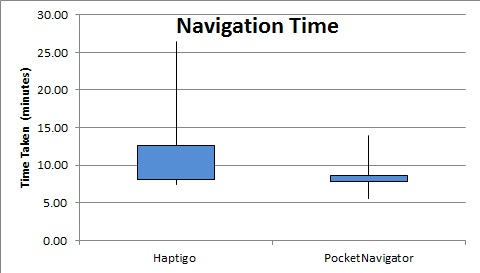
\includegraphics[width=0.8\columnwidth]{Images/NavigationTime.jpg}
\label{figure:haptigo:navigationtime}
\caption{Distribution of navigation time across ten particpants.}
\end{figure}
    
\begin{figure}[ht]
\centering
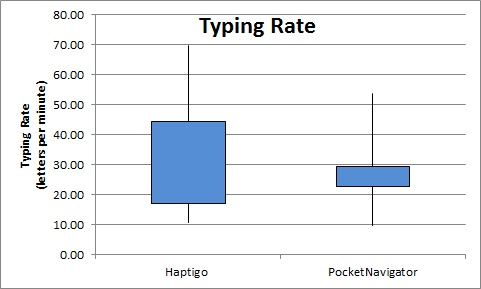
\includegraphics[width=0.8\columnwidth]{Images/TypingRate.jpg}
\caption{Distribution of typing rate across ten participants.}
\label{figure:haptigo:typingrate}
\end{figure}

The mean and standard deviation for user ratings on ease of use of the system and directional cues provided by the system are provided in Table \ref{table:haptigo:directioncues}. Figure[] shows the distribution of user ratings for Haptigo Direction Cues and Figure[] shows the distribution for PocketNavigator\cite{2010_Pielot_MobileHCI} Direction Cues. Five users stated that the haptigo system detected obstacles. Other users stated that they did not run into any obstacle during the navigation. Two users stated that there was one instance where the system alerted the user when there was no obstacle.

\begin{table}[ht]
  \small
  \centering
  \begin{tabular}{|c|c|c|}
    \hline
    \tabhead{Directional Cues} & Haptigo (Mean / SD) & PocketNavigator (Mean / SD) \\
    \hline
    Left & 4.2 / 1.03 & 4 / 1.24\\
    \hline
    Right & 4.2 / 1 & 3.8 / 1.22\\
    \hline
    Straight & 3.6 / 0.84 & 4 / 1.33\\
    \hline
  \end{tabular}
  \caption{Mean / Standard Deviation of directional haptic cues for Haptigo and PocketNavigator.}
  \label{table:haptigo:directioncues}
\end{table}

\begin{figure}[ht]
\centering
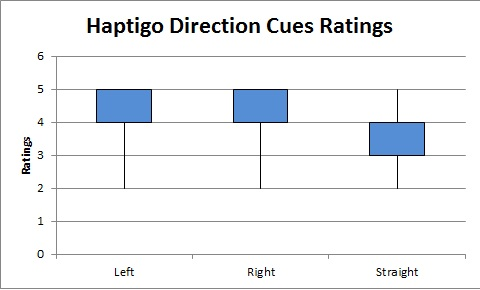
\includegraphics[width=0.8\columnwidth]{Images/HaptigoDirectionCueRatings.jpg}
\label{figure:haptigo:userratings}
\caption{Distribution of user ratings for direction cues of Haptigo.}
\end{figure}
    
\begin{figure}[ht]
\centering
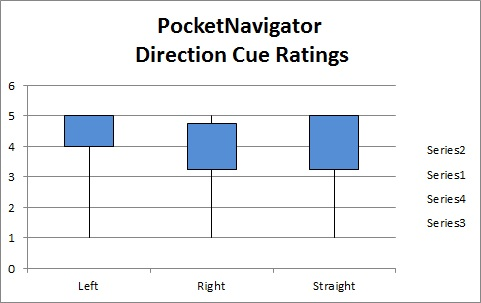
\includegraphics[width=0.8\columnwidth]{Images/PocketNavigatorDirectionCueRatings.jpg}
\caption{Distribution of user ratings for direction cues of PocketNavigator.}
\label{figure:pocketnavigator:userratings}
\end{figure}
% ##############################
% # DISCUSSION
% ##############################

\section{DISCUSSION}
The users were able to perform the navigation task without any mistakes. The users could perceive the directional and obstacle cues easily. The users noted that the strength of the haptic cue for the straight direction in the Haptigo was weak; it was difficult to perceive the vibrational signal. This is because the vibrational tactor for the straight direction is located just above the dip in the spinal region of the back. This tactor does not touch firmly against the body and thus is thus imperceptible to users. This can be remedied by substituting two vibrational tactors in place one for straight direction cue to make the vibrational signal stronger. The vibrational tactors could also be moved away from the center dip in the back in order to increase their strength.

The analysis of data collected from the user study showed that the performance of Haptigo was on par with the PocketNavigator\cite{2010_Pielot_MobileHCI}. The average navigation time for users with Haptigo (11.32 minutes) was higher than the navigation time for PocketNavigator\cite{2010_Pielot_MobileHCI}. The Paired T - Test on navigation times for the Haptigo and PocketNavigator\cite{2010_Pielot_MobileHCI} Systems shows that T(alpha < 0.05) = 0.15. Thus, the navigation time differences reported above were not statistically significant.

The average typing rate for a user using Haptigo (31.6 letters per minute) was greater than typing rate of the same user using PocketNavigator\cite{2010_Pielot_MobileHCI} (26.7 letters per minute). Paired T - Test for typing rate shows that T(alpha < 0.05) = 0.42. The typing rate differences were not statistically significant. The performance of Haptigo could not be proved to be neither better nor worse than PocketNavigator\cite{2010_Pielot_MobileHCI}. User’s rating for the directional cues for both systems were similar. Paired T - Test on user ratings for left , right and straight directional cues (T(alpha< 0.05)) are 0.69, 0.42 and 0.30. The user ratings for directional cues used in Haptigo and PocketNavigator\cite{2010_Pielot_MobileHCI} were not statistically different.

While using PocketNavigator\cite{2010_Pielot_MobileHCI}, One of the users asked the experimenter to alert him of any approaching obstacle since he was occupied with the task. The significant difference between both the systems is the awareness of the user’s environment provided by Haptigo. The average user rating for the haptic cues for obstacles was 4 with a standard deviation of 1.3. The cause for this deviation is attributed to a low rating for the haptic cues for obstacle avoidance. This low rating stemmed from the feedback of a user who was presented with a haptic cue for obstacle avoidance when there was no relevant obstacle within the immediate vicinity.

Five users stated that they were alerted of an approaching obstacle in the path while using Haptigo. Two users stated there were alerts of an obstacle when there were none in the path. This could be caused due to a wrong sensor reading. These instances were infrequent and had minimal influence on the overall navigation task. One user stated that the Haptigo system did not notify her when she walked into the low lying branch of a tree. We attribute this error to the limitations of ultrasonic sensors. Objects smaller in size (like thin tree branches) can often be missed as they do not present a large enough area to reflect the the initial incident pulse transmitted by the ultrasonic sensors. This limitation can be managed by approaching the object.

% ##############################
% # FUTURE WORK
% ##############################

\section{FUTURE WORK}
There were two concerns stated by the participants of the user study. One is the weak direction haptic cue for going straight and the other is the false positive in error detection. We would like to address the first concern by replacing one tactor in the lower back with two tactors and placing it equidistant from the center of the back. This would ensure that the vibrational tactors touch the user firmly in the back and the straight haptic cue is strong enough to be perceived. 

% ##############################
% # CONCLUSION
% ##############################

\section{CONCLUSION}
We have designed a wearable computing device which can act as a navigational aid for the user and maintain user’s awareness about his/her environment by detecting approaching obstacles. The users could perform the navigation task and identify obstacles after performing a calibration task and without a training. The position of the vibrational tactors and haptic cue presented were intuitive for the navigation and obstacle detection. We performed a user study with ten users to compare the performance of Haptigo as a navigational aid when compared to PocketNavigator\cite{2010_Pielot_MobileHCI}. For this sample of users, we found that the performance of Haptigo system was in par with PocketNavigator\cite{2010_Pielot_MobileHCI} in terms of navigation time and text typing rate. The advantage of using Haptigo system is provides awareness about the user’s environment by detecting approaching obstacles.

% Balancing columns in a ref list is a bit of a pain because you
% either use a hack like flushend or balance, or manually insert
% a column break.  http://www.tex.ac.uk/cgi-bin/texfaq2html?label=balance
% multicols doesn't work because we're already in two-column mode,
% and flushend isn't awesome, so I choose balance.  See this
% for more info: http://cs.brown.edu/system/software/latex/doc/balance.pdf
%
% Note that in a perfect world balance wants to be in the first
% column of the last page.
%
% If balance doesn't work for you, you can remove that and
% hard-code a column break into the bbl file right before you
% submit:
%
% http://stackoverflow.com/questions/2149854/how-to-manually-equalize-columns-
% in-an-ieee-paper-if-using-bibtex
%
% Or, just remove \balance and give up on balancing the last page.
%
\balance

% If you want to use smaller typesetting for the reference list,
% uncomment the following line:
% \small
\bibliographystyle{acm-sigchi}
\bibliography{paper}
\end{document}
